\documentclass[a4paper,titlepage,12pt,twoside,openright]{scrreprt}

\usepackage{fancyref}
\usepackage{multirow}
\usepackage{tikz}
\usetikzlibrary{trees}
\usetikzlibrary{shapes}
\usepackage{listings}

% Include style for title page, legal clause, and required classes.
% Also sets the page style, header and footer.
\usepackage{cappstyle}

% So we have bold style tt font.
\usepackage{courier}

% Enter your hyphenation list, i.e. hy-phe-na-tion, in order to have these
% words hyphenated correctly at the end of a line. Use spaces to separate 
% words.
\hyphenation{}

\begin{document}

	% make empty pages clear without any header, without any footer
    \pagestyle{empty}

    \capptitle{Studienarbeit}
         {}                         % nuber of this thesis, normally blank
         {Fast~and~Exact~Floating-Point~Accumulation}  % title of thesis
         {Reimar~D�ffinger}                % author name
         {Dr.~Rainer~Buchty} % supervisor
         {M�rz 2008}        % month & year (for title page)
         {Reimar D�ffinger\\ 
          Schauinslandstr. 4\\ 
          75249 Kieselbronn\\ 
          email: Reimar.Doeffinger@gmx.de}     % address
          {Prof.~Dr.~Wolfgang~Karl}
          
    \cappclause{Reimar D�ffinger}          % author name
         {Karlsruhe, 01.03.2008}    % location, date (for legal clause)


    % reset parskip to more useful settings than 1.5ex as in cappstyle.sty
    \setlength{\parskip}{1.45ex plus 0.5ex minus 0.2ex}

    \cleardoublepage
    % Abstract
    \begin{abstract}
  \begin{center}
    \textbf{\abstractname}
  \end{center}
\end{abstract}

    \cleardoublepage

    \pagenumbering{Roman}
    \pagestyle{plain}
    \tableofcontents
    \listoftables
    \listoffigures
    \cleardoublepage

	\pagestyle{myfancy}
    % include this numbering in this file as it does not work when directly 
% including in Dokument.tex
\pagenumbering{arabic}

\chapter{Motivation}
It is well known that the ever increasing computing speed allows more
and more problems to be solved computationally.
But it also means --- especially with iterative algorithms --- that problems
that could already be solved before can now be solved with higher accuracy.
Thus, calculations can now much more easily hit the accuracy limit of the
computer's native number format --- usually IEEE 754 double precision floating
point.
There are several solutions to this. One is to just increase the size of the
floating point format once again, as when switching from single- to
double-precision (a switch, that in case of Cell or GPU processing is still in
progress).
Another is full software emulation of larger data types as e.g. the
MPFR library~\footnote{\url{http://www.mpfr.org}} provides.\\
The approach used here instead is based on the previous work by
Dr. Ulrich W. Kulisch~\cite{advar} and --- while keeping the current native
floating point numbers --- implements additional, exact operations on these.
Compared to just increasing the size of floating point numbers this has the
advantage that at least some operations will be exact, and thus there is no
need for an error estimation on these, which is a big advantage since error
estimation is difficult and imprecise when done on a theoretical level
beforehand and slow and often still imprecise when done during runtime e.g.
via intervall arithmetic.
Compared to a full software implementation it is still very well implementable
in hardware, thus allowing for much faster speed.\\
In the following, only an exact accumulation operation on single precision floating
point numbers and its implementation is presented.\\
Extending the design to support double precision should be a question of solving
some minor, but time consuming technical issues due to e.g. HyperTransport data
unit size being only 32 bit.\\
Contrary to the work by Dr. Kulisch, multiplication was not implemented since
multipliers on FPGAs especially for large sizes can simply not compete with
those in a modern CPU and would use up a lot of hardware resources even if
a user might have more use for e.g. square-root-and-accumulate than
multiply-and-accumulate.



    \chapter{Basic HyperTransport Concepts}

To ease understanding of some of the implementation approaches, I will describe
some of the basics of HyperTransport and some of the details that are not easy
find elsewhere.\\
For more details and precise descriptions, please refer to the HyperTransport
specification~\cite{htspec}.\\
HyperTransport is a high-speed device interconnect, used in particular by AMD
CPUs.\\
A HyperTransport link always connects exactly two devices, which means reduced
management overhead compared to and ordinary bus, while still allowing to
connect many devices by allowing chaining of links, tunnels and bridges.\\
An optional part of the specification also allows for more complex
HyperTransport networks with more advanced routing.\\
On the physical level, HyperTransport uses differential signalling and
independent links for each communication direction.\\
Link speed can be varied independently in each direction as well, allowing
any combination of link frequencies from 200 to 2600 MHz (DDR) and link widths
of 2 bits to 32 bits (requiring 29 to 199 pins respectively~\cite{htarch}).\\
Each link also uses 3 independent virtual channels (i.e. each has their own
buffers so they can not block each other): posted, nonposted and response.\\
Flow control is done using a credit-based system: each virtual channel has an
associated number of credits on the sender side (representing available buffers
on the receiver side), independent for command and data.\\
Sending a command/data reduces the number of credits on the sender side,
the receiver increases them again by sending appropriate nop command packets
(nops do not use credits, thus no deadlocks are possible).\\
For data, each data packet uses one credit (size can vary between 4 and 64
bytes).\\
There is an optional data credit mode where each 4 bytes of data use up one
credit, but this is not available in the implementation used.\\
The implementation used provides 32 credits for each virtual channel, for both
command and data.\\
HyperTransport devices are configured (e.g. base address) by a set of registers
with same layout and behaviour as PCI configuration registers, so it is easily
possible to use a HyperTransport device just like a PCI device, just with a much
faster and lower latency connection.\\

    \chapter{Components of the Hardware Design}

This chapter gives an overview of the general design of the hardware
part of the system, which should help understanding the code.
Additional details are available as source-code comments which
can also be extracted into a separate document via
doxygen~\footnote{\url{http://www.stack.nl/~dimitri/doxygen/}}.
Note that at least version 1.5.5 is needed since previous versions
do not support VHDL.\\

\begin{figure}[ht]
\begin{center}
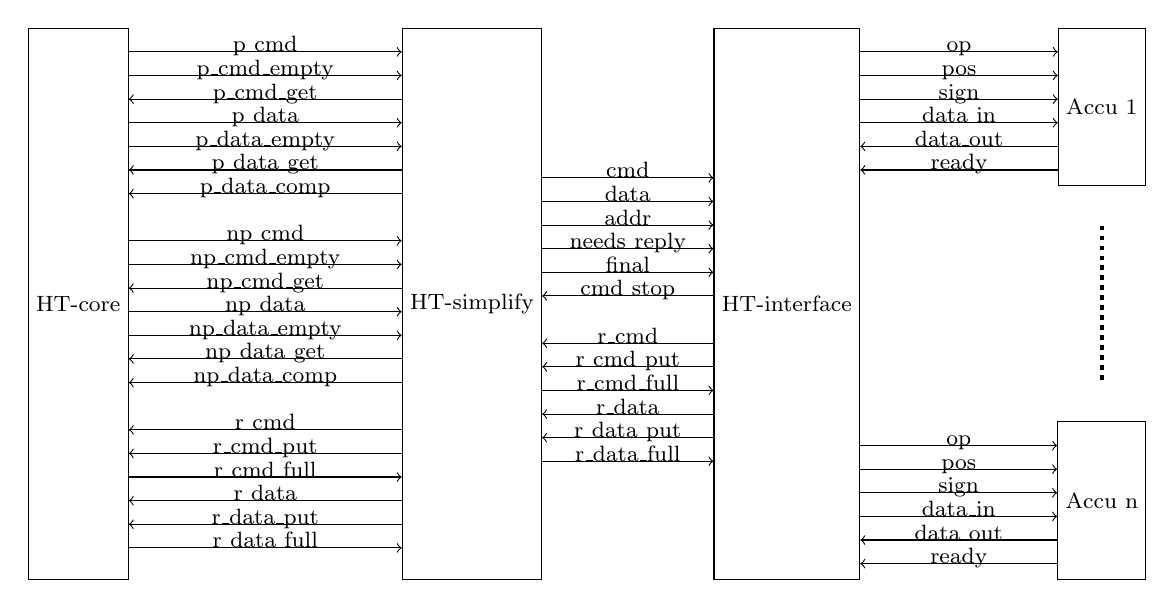
\begin{tikzpicture}
  \footnotesize
  \tikzstyle{every node}=[rectangle,draw]
  \node[minimum height=7cm] (HT-core)      at (0   ,0) {HT-core};
  \node[minimum height=7cm] (HT-simplify)  at (50mm,0) {HT-simplify};
  \node[minimum height=7cm] (HT-interface) at (90mm,0) {HT-interface};
  \node[minimum height=2cm] (acc1) at (130mm,+25mm) {Accu 1};
  \node[minimum height=2cm] (accn) at (130mm,-25mm) {Accu n};
  \tikzstyle{dots}=[dotted,ultra thick]
  \draw[dots,shorten >=5mm,shorten <=5mm] (acc1) -- (accn);

%% draw connections
  \tikzstyle{every node}=[pos=0.5,draw=none,anchor=base]

%% core <-> simplifier connections
  \newcommand{\mysc}{-3mm}
  \newcommand{\myofs}{32mm}
  \foreach \n/\txt in {  0/p\_cmd,   1/p\_cmd\_empty,   3/p\_data,   4/p\_data\_empty,
                         8/np\_cmd,  9/np\_cmd\_empty, 11/np\_data, 12/np\_data\_empty,
                        18/r\_cmd\_full, 21/r\_data\_full}
    \draw[->] ([yshift=\mysc*\n+\myofs] HT-core.east) -- ([yshift=\mysc*\n+\myofs] HT-simplify.west) node {\txt};
  \foreach \n/\txt in {  2/p\_cmd\_get,   5/p\_data\_get,   6/p\_data\_comp,
                        10/np\_cmd\_get, 13/np\_data\_get, 14/np\_data\_comp,
                        16/r\_cmd,       17/r\_cmd\_put,   19/r\_data,        20/r\_data\_put}
    \draw[<-] ([yshift=\mysc*\n+\myofs] HT-core.east) -- ([yshift=\mysc*\n+\myofs] HT-simplify.west) node {\txt};

%% simplifier <-> mmap interface connections
  \renewcommand{\mysc}{-3mm}
  \renewcommand{\myofs}{16mm}
  \foreach \n/\txt in {  0/cmd, 1/data, 2/addr, 3/needs\_reply, 4/final,
                         9/r\_cmd\_full, 12/r\_data\_full}
    \draw[->] ([yshift=\mysc*\n+\myofs] HT-simplify.east) -- ([yshift=\mysc*\n+\myofs] HT-interface.west) node {\txt};
  \foreach \n/\txt in {  5/cmd\_stop,
                         7/r\_cmd,        8/r\_cmd\_put,   10/r\_data,        11/r\_data\_put}
    \draw[<-] ([yshift=\mysc*\n+\myofs] HT-simplify.east) -- ([yshift=\mysc*\n+\myofs] HT-interface.west) node {\txt};

%% mmap interface <-> accumulators connections
  \renewcommand{\mysc}{-3mm}
  \renewcommand{\myofs}{7mm}
  \foreach \n/\txt in {  0/op, 1/pos, 2/sign, 3/data\_in} {
    \draw[->] ([yshift= 25mm+\mysc*\n+\myofs] HT-interface.east) -- ([yshift=\mysc*\n+\myofs] acc1.west) node {\txt};
    \draw[->] ([yshift=-25mm+\mysc*\n+\myofs] HT-interface.east) -- ([yshift=\mysc*\n+\myofs] accn.west) node {\txt};
  };
  \foreach \n/\txt in {  4/data\_out, 5/ready} {
    \draw[<-] ([yshift= 25mm+\mysc*\n+\myofs] HT-interface.east) -- ([yshift=\mysc*\n+\myofs] acc1.west) node {\txt};
    \draw[<-] ([yshift=-25mm+\mysc*\n+\myofs] HT-interface.east) -- ([yshift=\mysc*\n+\myofs] accn.west) node {\txt};
  };
\end{tikzpicture}.

\end{center}
\caption{Modules and basic architecture of the design}
\label{fig:modules}
\end{figure}

The system consists of 4 distinct parts, each implemented as a
separate VHDL entity (except the HyperTransport core which is written in
Verilog), as shown in~\fref{fig:modules}.\\
The connections between these four parts and also connection between the
HyperTransport core and the FPGA pins are described in a toplevel module
called "acctop" which is not depicted since it only contains connections
and no relevant code of its own.\\
Each of these parts are described in detail in the following sections.

\section{The HyperTransport Core}

The HyperTransport implementation used originally is the "HT Core" by the
Computer Architecture Group of the University of Mannheim~\cite{htcore},
more specifically the version 0.9 for 16-bit links from September 2007.
Unfortunately, that version has some problem that causes HyperTransport
transfers to be very slow, reducing the speed by more than a factor 3.
In addition, it also uses a port named reset\_\_n, but consecutive
underscores are not allowed in VHDL and thus this port must be renamed
before it can be used via VHDL.\\
Thus using the version 1.0 is strongly recommended, although it has
a slightly different usage and there is no documentation at all available
for it --- though at least the ucf restraint file can be reused from
the version 0.9 example code.
Make sure to correctly configure this core by modifying the htcore\_params.h
file, in particular make sure HT\_CORE\_INDEPENDENT\_CLK is defined,
for a "final" design, setting the PCI vendor and device IDs and the
PCI BAR0\_SIZE to better values than the default is advisable as well.\\
Finally, as these implementations handle HyperTransport data credits in a
non-trivial way, and since its documentation does not explain this clearly, it is
explained here.\\
Credits for commands are restored to the sender automatically when they are
read from the fifo, whereas for data (since it can have varying size) an
explicit data\_complete signal must be used.\\
This signal must be set to high for exactly one cycle each time a data packet
has been completely read. In particular, it must not be set if a command
has no associated data, and it must be set for only one cycle even if reading
all associated data takes multiple cycles, and it must be set after or
exactly when the last data of the packet is shifted out of the FIFO.\\
Since correct handling of this signal increases complexity significantly
and wrong handling can result in the CPU hanging, this together with some
additional simplifications is handled separately in the ht\_simplify module,
described in~\fref{sec:htsimplify}.

\section{The HyperTransport Simplification Layer}
\label{sec:htsimplify}

The HyperTransport simplification layer (the module called ht\_simplify)
merges the posted and non-posted queue into one queue, handles setting
the data\_complete signals of the HyperTransport core, splits multi-dword
reads/writes into multiple reads/writes of a single dword and inserts nop
commands into the queue as necessary, thus eliminating the need for
and extra "empty" signal, and provides a signal that indicates
if the current command must be replied to via the response queue.\\
There is also a "final" signal that is necessary to handle correctly
split reads: all responses up to when the "final" signal is set
must be answered in one single response packet.\\
The "final" signal is set for other commands as well, but it should
not be necessary there (it might help implement correct handling
of byte-sized, masked writes though).\\
This greatly reduces the complexity and frustration of designing a device
that uses HyperTransport by handling the parts that are most error-prone
and easily lead to a stopped CPU.\\
In the current implementation it has also several drawbacks: byte-sized
writes are not handled correctly, and the transfer rate is limited to one command
and 32 bits data per clock cycle, whereas the HT Core allows for up to one
command and 64 bits of data per clock cycle per queue.\\

\section{The Memory-Mapping Interface}

The memory-mapping interface translates HyperTransport read-/write-requests into
operations on the ALUs.\\
Each ALU is assigned its own 4KB address space. The 4KB size was chosen to allow
managing the ALUs via the CPUs MMU.
This allows arbitrary mapping of ALU number as seen by the software to hardware
ALU number, thus e.g. two programs each using ALUs 0 -- 4 in their code can be remapped
via MMU for one to use ALUs 0 -- 4 and the other 5 -- 8, so that no expensive saving and
restoring of ALU state is necessary on program switches.\\
This functionality would need a kernel-level driver though, currently there is only
a purely user-level library available for accessing the functionality.\\

\begin{figure}[ht]
\begin{center}
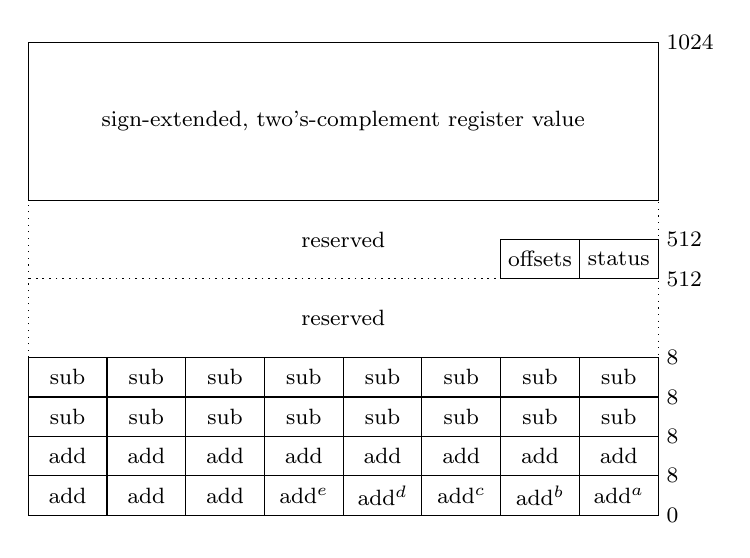
\begin{tikzpicture}
  \footnotesize
  \newcommand{\rectw}{10mm}
  \newcommand{\recth}{5mm}
  \newcommand\drawblock[3]{\draw (#1*\rectw,#2*\recth) rectangle +(\rectw,\recth);\draw (#1*\rectw+\rectw/2,#2*\recth+\recth/2) node {#3};}
  \newcounter{addr}
  \draw (8*\rectw,0*\recth) node[right] {0};
  \drawblock{0}{0}{add}
  \drawblock{1}{0}{add}
  \drawblock{2}{0}{add}
  \drawblock{3}{0}{add$^e$}
  \drawblock{4}{0}{add$^d$}
  \drawblock{5}{0}{add$^c$}
  \drawblock{6}{0}{add$^b$}
  \drawblock{7}{0}{add$^a$}
  \foreach \y/\text in {1/add,2/sub,3/sub}{
    \setcounter{addr}{8*\y}
    \draw (8*\rectw,\y*\recth) node[right] {\arabic{addr}};
    \foreach \x in {0,...,7}{
      \drawblock{\x}{\y}{\text}
    }
  }
  \setcounter{addr}{8*4}
  \draw (8*\rectw,4*\recth) node[right] {\arabic{addr}};

% reserved command part
  \draw[style=dotted] (0*\rectw,4*\recth) rectangle +(8*\rectw,2*\recth);
  \draw (4*\rectw,5*\recth) node {reserved};

  \draw (8*\rectw,6*\recth) node[right] {512};
% status flags/offsets part
  \drawblock{7}{6}{status}
  \drawblock{6}{6}{offsets}
  \setcounter{addr}{512+8}
  \draw (8*\rectw,7*\recth) node[right] {\arabic{addr}};

% reserved status part
  \draw[style=dotted] (0*\rectw,6*\recth) rectangle +(8*\rectw,2*\recth);
  \draw (4*\rectw,7*\recth) node {reserved};

% main register
  \draw (0*\rectw,8*\recth) rectangle +(8*\rectw,4*\recth);
  \draw (4*\rectw,10*\recth) node {sign-extended, two's-complement register value};
  \draw (8*\rectw,12*\recth) node[right] {1024};

\end{tikzpicture}

\label{fig:memlayout}
\caption{Memory layout for memory-mapped access to ALUs}
\begin{tabular}{ll}
$^a$ & read: current ALU value as float rounded to $0$\\
$^b$ & read: current ALU value as float rounded away from $0$\\
$^c$ & read: current ALU value as float rounded to $-\infty$\\
$^d$ & read: current ALU value as float rounded to $+\infty$\\
$^e$ & read: current ALU value as float rounded to nearest\\
\end{tabular}
\end{center}
\end{figure}

The memory layout of a single ALU is described in~\fref{fig:memlayout}.
Address offsets are indicated on the right side in multiples of 4 bytes.\\
The 4 KB area is split in two 2 KB parts: the lower part to execute operations
on the ALU and the upper part for the status.\\
For the command area only areas that add or subtract the written single-precision
floating-point value and the five blocks marked $^a$ to $^e$ that on read
return the current value as a single-precision floating-point value with different
rounding modes are defined.\\
There many consecutive 32-bit blocks that have the same functionality
(add or subtract) since this allows for write-combining and thus better
utilization of HyperTransport bandwidth.\\
The complete ALU status can be saved and restored simply by reading and writing
the upper 2 KB, starting with the lowest address. Note that since byte-sized
writes are not implemented by the HyperTransport interface you should avoid
using normal memory copy functions like memcpy in C and instead use your own
function that always reads and writes 32 bit blocks or multiples thereof.\\
The meaning of the offset and status blocks in the status area are explained
in~\fref{sec:aluops} under op\_readoffset, op\_writeoffset, op\_readflags
and op\_writeflags.\\
Large parts of both areas are reserved for future extensions, like support for
double precisions, multiply-and-accumulate or even more advanced operations.\\

    \chapter{The ALU core}
\section{Interface of the Accumulator VHDL Entity}
\subsection{Ports of the ALU Core}
\newcommand\tabhead[1]{\hline\multicolumn{2}{|c|}{#1}\\ \hline}
\newcommand\tabline[2]{#1 & #2\\ \hline}
\begin{center}
\begin{tabularx}{\textwidth}{|l|X|}
\tabhead     {Basic input signals}
\tabline {clock}     {sensitive to rising edge.}
\tabline {reset}     {set to 1 for an (asynchronous) reset.}
\hline
\tabhead     {Control input signals}
\tabline {sign}      {set to 1 for subtraction instead of addition (flip sign).}
\tabline {op}        {operation to execute. Use one of the op\_ constants.}
\tabline {data\_in}  {data to operate on.}
\tabline {pos}       {block position as signed value needed for some operations.}
\hline
\tabhead     {Output signals}
\tabline {ready}     {
        if 1 indicates that the operation given by the control input signals
        is now being processed and the control input signals should be set to
        the right values for the next operation.
        Use op\_nop if you do not have any next operation to execute (yet).
        The input signals may be changed at any time, not only when ready
        is 1, any value when ready was not 1 will be ignored.}
\tabline {data\_out} {
        result data after any read operation. This will be valid the
        cycle after the ready signal becomes 1 to indicate the start of
        processing for the operation following the read.}
\end{tabularx}
\end{center}

\subsection{Operations of the ALU Core}
\label{sec:aluops}
\renewcommand\tabline[2]{#1 & #2\\ \hline}
\begin{center}
\begin{tabularx}{\textwidth}{|l|X|}
\hline
\tabline {Name}  {Function}
\hline
\tabline {op\_nop} {no operation, idle}
\tabline {op\_add} {
    add/subtract (depending on sign signal) a 64 bit block
    (representing a positive integer) at the 32 bit block offset
    specified by the pos signal.}
\tabline {op\_readblock} {
    read 32 bit block specified by the pos signal, reads
    below the actually RAM-backed memory range return 0,
    reads above 0 for positive, X"FFFFFFFF" for negative values.}
\tabline {op\_writeblock} {
    write 32 bit block specified by the pos signal, writes outside
    the implemented range are ignored (ideally they should set overflow/
    underflow flags as appropriate).}
\tabline {op\_readflags} {
    read virtual 32 bit flag register. The upper 16 bits indicate
    which of the lower 16 bits (the actual flags) are valid, which
    allows for compatibility with future extended versions.
    For a list of currently available flags see~\fref{tab:flags}.}
\tabline {op\_writeflags} {
    set the flags marked by a set bit in the upper 16 bits to
    the value in the lower 16 bits.
    This is mostly for allowing to restore the register state from system
    RAM and rarely useful otherwise.
    For a list of available flags see~\fref{tab:flags}.}
\tabline {op\_readoffsets} {
    get exponent offsets for floating point operations.
    Exponent offsets are two 16 bit signed integers.
    Lower 16 bits are for writes (op\_floatadd) higher 16 bits for reads (op\_readfloat).}
\tabline {op\_writeoffsets} {
    set exponent offsets for floating point operations.
    Exponent offsets are two 16 bit signed integers.
    Lower 16 bits are for writes (op\_floatadd) higher 16 bits for reads (op\_readfloat).}
\tabline {op\_readfloat} {
    reads the current register content as a single-precision
    floating-point value. Denormals and $\pm\infty$ are supported, values that should
    be NaN are returned as $\pm\infty$.
    The pos signal is misused to specify the rounding mode, see~\fref{tab:round}.}
\tabline {op\_floatadd} {
    adds/subtracts (depending on sign signal) the given
    single-precision floating-point value. Note that NaN is treated as $\infty$
    currently.}
\end{tabularx}
\end{center}

\begin{table}[ht]
\label{tab:round}
\renewcommand\tabline[2]{#1 & #2\\ \hline}
\begin{center}
\begin{tabular}{|l|l|}
\hline
\tabline {pos signal} {rounding mode}
\hline
\tabline {0}          {to $0$}
\tabline {1}          {away from $0$}
\tabline {2}          {to $-\infty$}
\tabline {3}          {to $+\infty$}
\tabline {4}          {to nearest}
\tabline {other}      {unspecified}
\end{tabular}
\caption{Rounding Modes}
\end{center}
\end{table}

\begin{table}[ht]
\label{tab:flags}
\renewcommand\tabline[2]{#1 & #2\\ \hline}
\begin{center}
\begin{tabular}{|r|l|}
\hline
\tabline {Bit} {Name}
\hline
\tabline {0}   {sign}
\tabline {1}   {overflow}
\tabline {2}   {zero}
\end{tabular}
\caption{ALU flags}
\end{center}
\end{table}

\subsection{The ALU Flags}

Currently, 3 flags are supported: sign, overflow and zero.\\
The sign and zero flags have their usual meaning, indicating if
the register value is negative or zero. Contrary to normal floating
point values, negative 0 does not exist.\\
Writing to the sign flag only changes the sign while keeping the two's
complement representation the same, so this has probably no practical
use beyond restoring the register state.\\
Clearing the zero flag has no effect, since there is no obvious and non-conflicting
way to give this a meaning. Setting the zero flag clears the register's two's
complement representation. This should always be combined with clearing the sign
flag, otherwise the behaviour (while still well-defined) might be unexpected,
and usually the overflow flag should be cleared as well.\\
The overflow flag indicates any kind of overflow-like situation: adding $\pm\infty$,
adding NaN, adding a value that is too large to fit into the backing RAM (e.g. due
to a large write exponent offset) or an addition that causes an ordinary overflow
of the two's complement representation.\\
By periodically checking and clearing the overflow flag it is possible to
detect summand ranges that contain $\infty$ or NaN values and process these
parts more carefully in an additional step. Note that to make this work well,
adding $\infty$ or NaN has \em no \rm effect except setting the overflow flag.\\
While the overflow flag is set, reads will return $\pm\infty$, after clearing
the flag the result will be the same as if there had been no $\pm\infty$ or NaN
value in the input.\\
In general, any operations that can cause the overflow flag to be set should ensure
that the register value is updated in a way that allows "chaining" of registers
to simplify extension to larger exponent ranges.\\
Chaining means that multiple registers add the same numbers, but use different
write exponent offsets. Like this, these registers together can be used
as one larger register with some additional (possibly software) code to handle
reading the current value.\\
An obvious future extension to these flags would be an "inexact" flag if due to
a negative write exponent offset or addition of double-precision support the
ALU is no longer always exact.

\section{Implementation details}
\subsection{Steps of the op\_floatadd Operation}

\renewcommand\tabline[2]{#1 & \multicolumn{5}{p{0.8\textwidth}|}{#2}\\}
\begin{center}
\begin{tabularx}{\textwidth}{|r|X|r|X|r|X|}
\hline
\tabline {  0} {Handle $\infty$/NaN special cases by setting the overflow bit}
\tabline {  1} {combine sign of value with sign signal}
\tabline {  2} {extract 32 bit block position and shift value from exponent}
\tabline {  3} {extract mantissa (with leading 1 or 0 depending on denormal or not)}
\tabline {  4} {shift mantissa for alignment with 32 bit block boundary}
\tabline {  5} {load first 32 bit block}
\tabline {  6} {add/subtract lower part of mantissa to block value}
\tabline {  7} {store first 32 bit block}
\tabline {  8} {load second 32 bit block}
\tabline {  9} {add/subtract upper part of mantissa and carry to block value}
\tabline { 10} {store second 32 bit block}
\hline\hline
\multicolumn{6}{|p{0.75\textwidth}|}{
    The following steps are only necessary if carry is set,
    but currently they are done always to simplify the implementation}\\
\hline\hline
\tabline { 11} {calculate carry resolution position}
\tabline { 12} {flip bits in-between current position and carry-resolution position}
\hline
13a & load 32 bit block for carry resolution &
\multirow{3}{*}{13b} & \multirow{3}{0.25\textwidth}{flip sign bit as part of carry resolution} &
\multirow{3}{*}{13c} & \multirow{3}{0.25\textwidth}{set overflow bit as part of carry "resolution"}\\
14a & add/subtract carry & & & &\\
15a & store 32 bit block for carry resolution & & & &\\
\hline
\end{tabularx}
\end{center}

These steps are organized into clock cycles as follows:\\
\renewcommand\tabline[3]{#1 & #2 & #3\\}
\begin{center}
\begin{tabular}{|r|l|l|}
\hline
\tabline {Clock} {Steps}                          {State}
\hline
\tabline {1}     {0) - 3)}                        {some final state}
\tabline {2}     {4), 5)}                         {st\_in\_float0}
\tabline {3}     {6), 8), 11), pre-calculate 12)} {st\_add1}
\tabline {4}     {7), 9), 13a)}                   {st\_add2}
\tabline {5}     {10), 12), 14a), 13b), 13c)}     {st\_fixcarry}
\tabline {6}     {15a)}                           {first of next command}
\hline
\end{tabular}
\end{center}
For descriptions of the states, see~\fref{sec:alustate}.\\

Note that processing of the next operation starts with Clock 5, so in
each 4 cycles one floatadd operation can complete.\\
Reducing the number of clock cycles is difficult for several reasons:\\
\begin{itemize}
\item Skipping carry resolution if there is no carry is probably easiest, but
      will increase code complexity since the carry value is only known after
      Clock 4, but to gain anything processing of the next instruction would
      have to start \em at \rm Clock 4.
\item The dual-port BlockRAM resource can not service more read-write requests
      than the current implementation uses, thus any improvements either need
      to use multiple BlockRAMs (which in a previous implementation resulted in
      low clock speeds) or a RAM resource with more than 2 ports.
\item Pipelining will need difficult dependency resolution, since the 32 bit blocks
      that are changed only become known for certain in step 12, though for the
      general case a worst-case guess based on the pre-calculated value for step
      12) may be good enough.
\end{itemize}

\subsection{Steps of the op\_readfloat Operation}

\begin{center}
\begin{tabularx}{\textwidth}{|r|X|}
\hline
 1 & Determine block number of highest set bit (highest bit not equal to sign),
     or the number of the block containing the lowest bit representable by a
     denormal if this is higher.\\
 2 & read block determined in step 1) and the one below.\\
 3 & determine position of first set/unset bit in read block.\\
 4 & calculate exponent value with information from steps 1) and 3).\\
 5 & use value from step 3) to shift the blocks read in 2) so that the highest
     bit unequal to the sign is "leftmost".\\
 6 & determine which is the lowest block that is not all 0.\\
 7 & use results of steps 5) and 6) to check if the value can be represented
     exactly as float, a special case for denormals needs exponent from step 4).\\
 8 & for negative values now invert the value from step 5) (together with rounding
     converts two's complement to absolute value for mantissa).\\
 9 & apply rounding if necessary (needs result from step 7) to avoid bias).\\
10 & adjust exponent for possible carry due to rounding.\\
11 & use sign, exponent from step 10) and mantissa from step 9) to build the float value.
     Needs special-case for denormals and infinities.\\
\hline
\end{tabularx}
\end{center}

These steps are organized into clock cycles as follows:\\
\renewcommand\tabline[3]{#1 & #2 & #3\\}
\begin{center}
\begin{tabularx}{\textwidth}{|r|l|X|}
\hline
\tabline {Clock} {Steps}                          {State}
\hline
\tabline {1}     {previous operation finishes}    {some final state}
\tabline {1a}    {wait if write-back pending}     {st\_out\_float0}
\tabline {2}     {1)}                             {st\_out\_float0}
\tabline {3}     {2), 6)}                         {st\_out\_float1}
\tabline {4}     {2), 3)}                         {st\_out\_float2}
\tabline {5}     {4)}                             {st\_out\_float3}
\tabline {6}     {4), 5), 7), 8)}                 {st\_out\_float4}
\tabline {7}     {9), 10), 11)}                   {st\_out\_float\_normal or st\_out\_float\_denormal or st\_out\_float\_inf}
\hline
\end{tabularx}
\end{center}
For descriptions of the states, see~\fref{sec:alustate}.\\

\subsection{State machine}
\label{sec:alustate}
\begin{figure}[ht]
\begin{center}
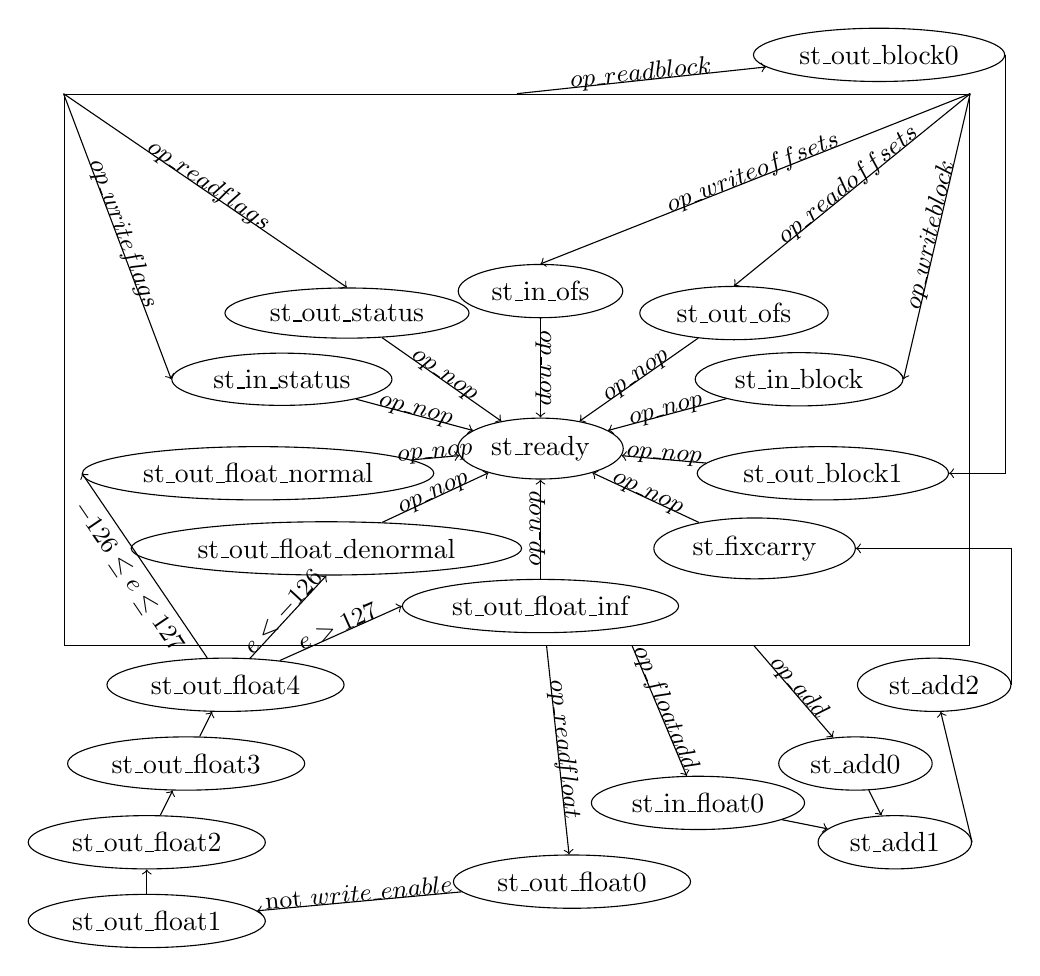
\begin{tikzpicture}
  \tikzstyle{every node}=[draw,shape=ellipse]
  \tikzstyle{op}=[midway,draw=none,sloped,anchor=base]
  \node[shape=rectangle, minimum width=11.5cm, minimum height=7cm] (finals) at (-3mm,1cm) {};
  \newcommand{\dist}{2cm}
  \node (ready)              at (0cm, 0mm)     {st\_ready};
  \node (fixcarry)           at (-25:30mm)     {st\_fixcarry};
  \node (out_block1)         at ( -5:36mm)     {st\_out\_block1};
  \node (in_block)           at ( 15:34mm)     {st\_in\_block};
  \node (out_ofs)            at ( 35:30mm)     {st\_out\_ofs};
  \node (in_ofs)             at ( 90:20mm)     {st\_in\_ofs};
  \node (out_status)         at (145:30mm)     {st\_out\_status};
  \node (in_status)          at (165:34mm)     {st\_in\_status};
  \node (out_float_normal)   at (185:36mm)     {st\_out\_float\_normal};
  \node (out_float_denormal) at (205:30mm)     {st\_out\_float\_denormal};
  \node (out_float_inf)      at (270:20mm)     {st\_out\_float\_inf};
  \foreach \src in {fixcarry,out_block1,in_block,out_ofs,in_ofs,out_status,in_status,
                    out_float_normal,out_float_denormal,out_float_inf}{
    \draw[->] (\src) -- (ready)                node[op] {\small $op\_nop$};
  }
% state transitions inside "final" states
  \draw[->] (finals.north east) -- (in_block.east)        node[op] {\small $op\_writeblock$};
  \draw[->] (finals.north east) -- (out_ofs.north)        node[op] {\small $op\_readoffsets$};
  \draw[->] (finals.north east) -- (in_ofs.north)         node[op] {\small $op\_writeoffsets$};
  \draw[->] (finals.north west) -- (out_status.north)     node[op] {\small $op\_readflags$};
  \draw[->] (finals.north west) -- (in_status.west)       node[op] {\small $op\_writeflags$};
% non-"final" states and transitions
  \node (out_block0)         at ( 43mm, 50mm)  {st\_out\_block0};
  \draw[->] (finals.north) -- (out_block0)     node[op] {\small $op\_readblock$};
  \draw[->] (out_block0.east) |- (out_block1);
  \node (add0)               at ( 40mm,-40mm)  {st\_add0};
  \draw[->] (finals) -- (add0)                 node[op] {\small $op\_add$};
  \node (in_float0)          at ( 20mm,-45mm)  {st\_in\_float0};
  \draw[->] (finals) -- (in_float0)            node[op] {\small $op\_floatadd$};
  \node (add1)               at ( 45mm,-50mm)  {st\_add1};
  \draw[->] (add0) -- (add1);
  \draw[->] (in_float0) -- (add1);
  \node (add2)               at ( 50mm,-30mm)  {st\_add2};
  \draw[->] (add1.east) -- (add2);
  \draw[->] (add2.east) |- (fixcarry);
  \node (out_float0)         at (  4mm,-55mm)  {st\_out\_float0};
  \node (out_float1)         at (-50mm,-60mm)  {st\_out\_float1};
  \node (out_float2)         at (-50mm,-50mm)  {st\_out\_float2};
  \node (out_float3)         at (-45mm,-40mm)  {st\_out\_float3};
  \node (out_float4)         at (-40mm,-30mm)  {st\_out\_float4};
  \draw[->] (finals) -- (out_float0)           node[op] {\small $op\_readfloat$};
  \draw[->] (out_float0) -- (out_float1)       node[op] {\small not $write\_enable$};
  \draw[->] (out_float1) -- (out_float2);
  \draw[->] (out_float2) -- (out_float3);
  \draw[->] (out_float3) -- (out_float4);
  \draw[->] (out_float4) -- (out_float_normal.west) node[op,below=-1mm] {\small $-126 \le e \le 127$};
  \draw[->] (out_float4) -- (out_float_denormal.south) node[op] {\small $e < -126$};
  \draw[->] (out_float4) -- (out_float_inf.west) node[op] {\small $e > 127$};
\end{tikzpicture}

\end{center}
\end{figure}


    \newcommand*{\fancyreflstlabelprefix}{lst}
\frefformat{vario}{\fancyreflstlabelprefix}{listing\fancyrefdefaultspacing#1#3}
\Frefformat{vario}{\fancyreflstlabelprefix}{Listing\fancyrefdefaultspacing#1#3}
\lstdefinelanguage[x86att]{Assembler}{
  morekeywords={
    add, addl, addq, call, clflush, enter, jmp, leave,
    mov, movaps, movl, movslq, movss, movq,
    pop, popl, push, pushl, ret, sal, sall, sub, subl, xor, xorl
  },
  morecomment=[l];,
  morecomment=[l]\#,
  morestring=[b]",
  morestring=[b]',
  keywordsprefix=\%
}

\chapter{The Software Interface}
For accessing the hardware a simple C library interface is provided.\\
Except for initialization most of the code is in the header file, so
that the functions can be inlined.\\
To demonstrate the difference this makes, the code in~\fref{lst:demo}
is compiled with different options.
All tests were done with "gcc (GCC) 4.1.2 (Ubuntu 4.1.2-0ubuntu4)".

%\lstset{basicstyle=\itshape}
\lstset{captionpos=b,columns=[c]flexible}
\lstset{language=C}
\begin{lstlisting}[float=ht,caption=compilation demonstration code,label=lst:demo]
#include "libefac.h"
void test(void) {
  efac_add4(0, 1.0, 1.0, 1.0, 1.0);
}
\end{lstlisting}

\lstset{language={[x86att]Assembler}}

\begin{lstlisting}[float=ht,caption={x86\_64 using register pointer (gcc -S -m64 -O3)},label={lst:regptr}]
test:
        movq    efac_regs(%rip), %rdx
        movl    $0x3f800000, %eax
        movl    %eax, 64(%rdx)
        movl    %eax, 68(%rdx)
        movl    %eax, 72(%rdx)
        movl    %eax, 76(%rdx)
        clflush 64(%rdx)
        ret
\end{lstlisting}

\begin{lstlisting}[float=ht,caption={x86\_64 inlined (gcc -S -m64 -O3)},label={lst:inline64}]
test:
        movl    $0x3f800000, %eax
        movl    %eax, efac_regs+64(%rip)
        movl    %eax, efac_regs+68(%rip)
        movl    %eax, efac_regs+72(%rip)
        movl    %eax, efac_regs+76(%rip)
        clflush efac_regs+64(%rip)
        ret
\end{lstlisting}

\begin{lstlisting}[float=ht,caption={x86\_64 not inlined (gcc -S -m64 -O3 -fno-inline)},label={lst:noinline64}]
efac_add4:
        sall    $12, %edi
        movslq  %edi,%rdi
        addq    $efac_regs, %rdi
        movss   %xmm0, 64(%rdi)
        movss   %xmm1, 68(%rdi)
        movss   %xmm2, 72(%rdi)
        movss   %xmm3, 76(%rdi)
        clflush 64(%rdi)
        ret

test:
        movss   .LC0(%rip), %xmm3
        xorl    %edi, %edi
        movaps  %xmm3, %xmm2
        movaps  %xmm3, %xmm1
        movaps  %xmm3, %xmm0
        jmp     efac_add4
\end{lstlisting}

\begin{lstlisting}[float=ht,caption={x86 inlined (gcc -S -m32 -O3)},label={lst:inline32}]
test:
        movl    $0x3f800000, %eax
        pushl   %ebp
        movl    %esp, %ebp
        movl    %eax, efac_regs+64
        movl    %eax, efac_regs+68
        movl    %eax, efac_regs+72
        movl    %eax, efac_regs+76
        clflush efac_regs+64
        popl    %ebp
        ret
\end{lstlisting}

\begin{lstlisting}[float=ht,caption={x86 not inlined (gcc -S -m32 -O3 -fno-inline)},label={lst:noinline32}]
efac_add4:
        pushl   %ebp
        movl    %esp, %ebp
        movl    8(%ebp), %edx
        sall    $12, %eax
        addl    $efac_regs, %eax
        movl    %edx, 64(%eax)
        movl    12(%ebp), %edx
        movl    %edx, 68(%eax)
        movl    16(%ebp), %edx
        movl    %edx, 72(%eax)
        movl    20(%ebp), %edx
        movl    %edx, 76(%eax)
        clflush 64(%eax)
        popl    %ebp
        ret

test:
        pushl   %ebp
        movl    $0x3f800000, %eax
        movl    %esp, %ebp
        subl    $16, %esp
        movl    %eax, 12(%esp)
        movl    %eax, 8(%esp)
        movl    %eax, 4(%esp)
        movl    %eax, (%esp)
        xorl    %eax, %eax
        call    efac_add4
        leave
        ret
\end{lstlisting}


    \appendix

    \chapter{HyperTransport Debugging}
Some HyperTransport errors cause a "machine check exception" (MCE) which
the Linux kernel will print as a message containing a hexadecimal
number.\\
And example of such a message is:\\
CPU 0: Machine Check Exception: 4 Bank 4 b200000000070f0f\\
This message can be translated into a clear-text string
with the mcelog program, for above message the result is:\\
\begin{verbatim}
> echo "CPU 0: Machine Check Exception: 4 Bank 4 b200000000070f0f" |\
  mcelog --k8 --ascii
HARDWARE ERROR. This is *NOT* a software problem!
Please contact your hardware vendor
CPU 0 4 northbridge   Northbridge ECC error
  ECC syndrome = 0
STATUS 0 MCGSTATUS 4
\end{verbatim}
This is an example that these messages are not always useful, since
an ECC error and a syndrom of 0 is usually contradictory.\\
A typical condition that causes an MCE is when the response
to a read request times out.\\
Unfortunately by far not all protocol errors cause an MCE. In particular,
answering a read request with "target done" (without data) instead of
a read request causes none, but results in "random" data as a result
of the read.
Note that it is usually not truly random but usually randomly one out of
about 4 different values with a strong bias towards one of those values
--- possibly whatever happened to be in the corresponding cache line or
register before.\\
There is also no error in case a read request for multiple dwords is only
responded with one single dword. This actually does not seem to cause
any problem at all. Unfortunately, the HyperTransport specification does
not say anything explicitly about this case, so it remains unclear if
this works just out of luck and with AMD's Opteron HyperTransport
implementation or if all HyperTransport devices must support this.\\



    \nocite{*}
%     \bibliographystyle{geralpha}
    \bibliographystyle{plain}
    \bibliography{Bibliografie}


\end{document}
